\chapter{BERT-Basierte Modelle}

In den letzten zwei Kapiteln wurde die Struktur des BERT-Models \ref{BERT}, sowie vom Transformer \ref{transformer},  vorgestellt. Diese können ausgebaut werden, um beliebige Aufgaben zu lösen. In diesem Kapitel stelle ich die entsprechenden Modelen vor, mit denen versucht wurde, Sätze in Leichte Sprache zu übersetzen. Die Struktur der Modele wird zuerst dargestellt und schließlich die Vorführung gegeben, wie diese Modele in Python eingesetzt werden können.

\section{Neural Machine Translation Model}
Das Neural Machine Translation Model (NMT-Model) ist eins der Komplexeren Modele, das in seinem Kern aus einem BERT-Model und einem Transformer besteht. Die Kombination der beiden Modelen bildet einen Supertransformer, sodass BERT und Transformer den NMT-Model aufbauen.

\subsection{Struktur des NMT-Model}
Die Struktur des Models ist durch die folgende Abbildung \ref{nmt_model_figure} gegeben:

\begin{figure}
	\centering
	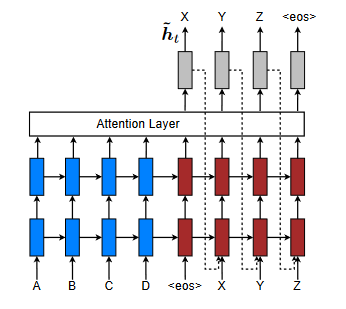
\includegraphics[scale=0.5]{images/NMT-Model.png}
	\caption{NMT-Model Struktur \cite{NMT:20}}
	\label{nmt_model_figure}
\end{figure}

Das BERT-Model wird für die Einbettung der Eingabe, welche Ausgabe in den Encoder und Decoder des Transformermodels später einfließt. Der Encoder muss somit keine eigene Einbettung für seine Eingabe berechnet, doch der Decoder muss seine eigene Einbettung berechnen. Für eine detailierte Erklärung der beiden Modellen kann als Referenz die früheren Kapitel benutzt werden (Kapitel \ref{Transformer}). Es wird jedoch der Fluß der Informationen hier gegeben:

Schritt-1: Bei einer Eingabe \textit{x} $\in$ \textit{X}, BERT bettet den \textit{x}-Vektor als $H_B = BERT(x)$ ein. Wo $H_B$ ist die Ausgabe des letzten Layers vom BERT. $h_{B,i} \in H_B$ stellt den \textit{i}-th Wort in x.

Schritt-2: Sei $H^l_E$ gegeben, was die Darstellung der versteckten \textit{l}-ten Schicht beschreibt und $H^0_E$ ist die Einbettung der Sequenz \textit{x}. Der \textit{i}-te Element aus $H^l_E$ wird als $h^l_i$ für $0<i<[l_x]$ definiert (begrenzt durch die Anzahl der Neuronen in jeder versteckten Schicht \textit{l}). Die Berechnung von $h^l_i$ ist gegeben:

\begin{equation}
	\tilde{h}^l_i = \frac{1}{2}(attn_S(h^{l-1}_i, H^{l-1}_E, H^{l-1}) + attn_B(h^{l-1}_i, H_B, H_B)), \text{ für } 0 < i < [l_x]
\end{equation}

Wo $attn_S$ und $attn_B$ sind Attention-Modele, bzw. MHA-Schichten, mit unterschiedliche Parametern (die Definition ist in Kapitel \ref{MHA_Layer} zu finden).

Weiterhin werden die berechneten Attentions nach ihrer Normierung dem Feed-Forward-Network gegeben und schließlich wird die Ausgabe normiert. Die Ausgabe aus der letzten Schicht ist durch $H^L_E$ definiert.

Schritt-3: die Eingabe im Decoder-Layer \textit{l} wird durch $S^l_{<t}$ für den Zeitpunkt \textit{t}, $S^l_{<t} = (s^l_1, · · · , s^l_{t−1})$. $s^0_1$ ist ein besonderer Zeichen, der den Anfang der Sequenz bestimmt und $s^0_t$ ist die Voraussage des Models zur bestimmten Zeitpunkt \textit{t}. Im Schicht \textit{l} erfolgt folgendes:	
\begin{subequations}
	\label{step_3}
\begin{gather}
	s^lt = attn_S (s^{l−1}t , S^{l−1}_{<t+1}, S^{l−1}_{<t+1})\\
	\~s^l_t = 1/2(attn_B (\ˆs^l_t, H_B , H_B ) + attn_E (\ˆs^l_t, H^L_E, H^L_E )), \text{ } s^l_t = FFN( ̃s^l_t)
\end{gather}
\end{subequations}


Die $attn_S$, $attn_B$ und $attn_E$ stellen entsprechend Self-, BERT-Decoder- und Encoder-Decoder-Attention dar. Eqn. \eqref{step_3} iteriert über die Schichten und liefert als Ergebnis $s^L_t$. Die Ausgabe fließt durch eine Dense-Schicht und schließlich mit einer Softmax-Funtion transformiert, sodass das t-te Wort $\^y_t$ erraten wird. Die Entschlusselung verläuft bis ein Endzeichen erreicht wird, bzw. bis die Ende der Sequenz verarbeitet wird. \cite{NMT:20}

\subsection{Implementierung}

Aus dem Artikel wird nicht genau klar, wie diese Model zu implementieren ist. Aus diesem Grund werden mehrere Versionen des Models versucht. Die Modele unterscheiden sich in der Embedding-Strategie. Das erste Model verwendent das BERT-Model für die Einbettung am Anfang und später im Decoder-Layer. Für die Implementierung werden die Bibliotheken \textit{tensorflow} und \textit{transformers} benutzt

